\documentclass{beamer}
\usepackage{graphicx}
\usepackage{subcaption}


%----------------------------------------------------------------------------------------
%	TITLE PAGE
%----------------------------------------------------------------------------------------

\title{Network Analysis of Tether Transactions}
\author{Yaejin Kim \inst{1} \and Matthias Hafner \inst{1,2}  \and  Philipp Pag \inst{1}}
\institute{   \inst{1} University of Zürich \and \inst{2} Center for Cryptoeconomics}
\date{\today}

\begin{document}


\begin{frame}
\titlepage % Print the title page as the first slide
\end{frame}

%------------------------------------------------

\begin{frame}{Introduction}
\framesubtitle{Motivation}

What is this study about?\\
 
     
\end{frame}

%------------------------------------------------

\begin{frame}{Data}
\framesubtitle{Dataset}


Lots of data.


\end{frame}




%------------------------------------------------

\begin{frame}{Pearson's correlation coefficient}
\framesubtitle{Background}	
	
	%Pearson's correlation coefficient $r$ is calculated as the co-variance of the two variables divided by the product of the standard deviation of each data sample as following:
	\begin{equation*}
		%\begin{split}
			%r = \frac{\sum(j_{out}-\overline{{j}_{out}})(k_{in}-\overline{{k}_{in}})}{L \sigma_{out}\sigma_{in}}
		%\end{split}
	\end{equation*}\\
	
\end{frame}

%------------------------------------------------

\begin{frame}{Theorem}
\framesubtitle{Test}		
	\begin{theorem}
		%Let \(f\) be a function whose derivative exists in every point, then \(f\) 
		is a continuous function.
	\end{theorem}
	
	
\end{frame}

%------------------------------------------------

\begin{frame} {Results I}
\framesubtitle{Highest Outdegree Nodes}			
	
	\begin{table}[!h]
		\scalebox{0.8}{%
			\centering
			\begin{tabular}{|c|c|c|c|}
				\hline
				\textbf{Address} & \textbf{Outdegree}& \textbf{Owner}\\ 
				\hline\hline
				0xab5c66752a9e8167967685f1450532fb96d5d24f & 120'100 & Huobi \\
				\hline
				0x1062a747393198f70f71ec65a582423dba7e5ab3 & 116'947 & Huobi \\ 
				\hline
				0x6748f50f686bfbca6fe8ad62b22228b87f31ff2b & 116'277 & Huobi \\
				\hline
				0xa8ae6549c66c59aa55d50377948dfbe362d56b03 & 76'408 & Unknown \\ 
				\hline
				0xfdb16996831753d5331ff813c29a93c76834a0ad & 58'710 & Huobi \\
				\hline
				0xadb2b42f6bd96f5c65920b9ac88619dce4166f94 & 55'207 & Huobi \\
				\hline
				0x0a98fb70939162725ae66e626fe4b52cff62c2e5 & 52'645 & Unknown \\
				\hline
				0xeee28d484628d41a82d01e21d12e2e78d69920da & 51'762 & Huobi \\
				\hline
				0x46705dfff24256421a05d056c29e81bdc09723b8 & 47'235 & Huobi \\
				\hline
				0xe93381fb4c4f14bda253907b18fad305d799241a & 44'917 & Huobi \\ 
				\hline
		\end{tabular}}
	\end{table}
	
\end{frame} 

%------------------------------------------------

\begin{frame} {Results II}
	\framesubtitle{Evolution of market prices}			
	
	\begin{figure}
		\centering
		\caption{Evolution of average market prices by treatment}
		\begin{subfigure}{.4\textwidth}
			\centering
			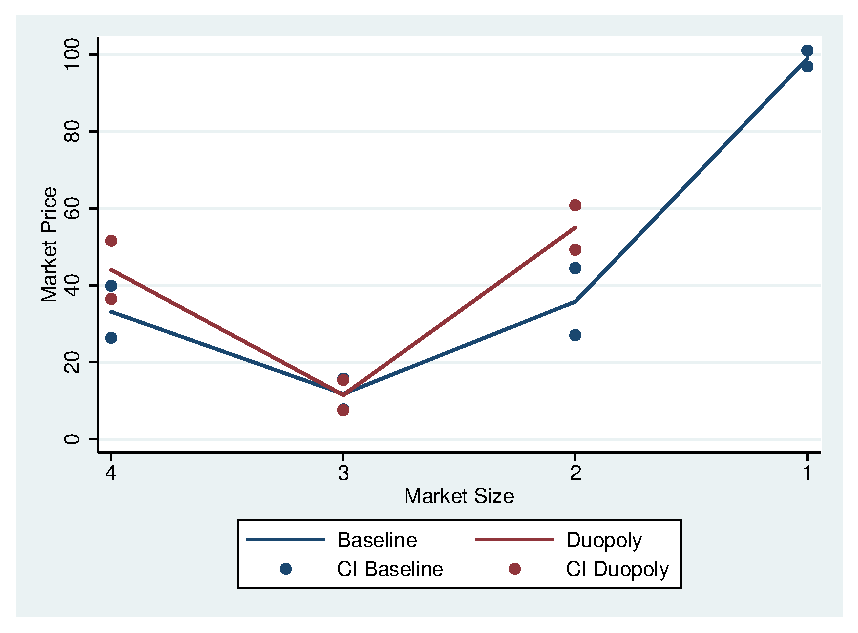
\includegraphics[width=0.9\linewidth]{market_price_on_market_size.eps}
			\caption{Price by market size}
		\end{subfigure}
		\begin{subfigure}{.4\textwidth}
			\centering
			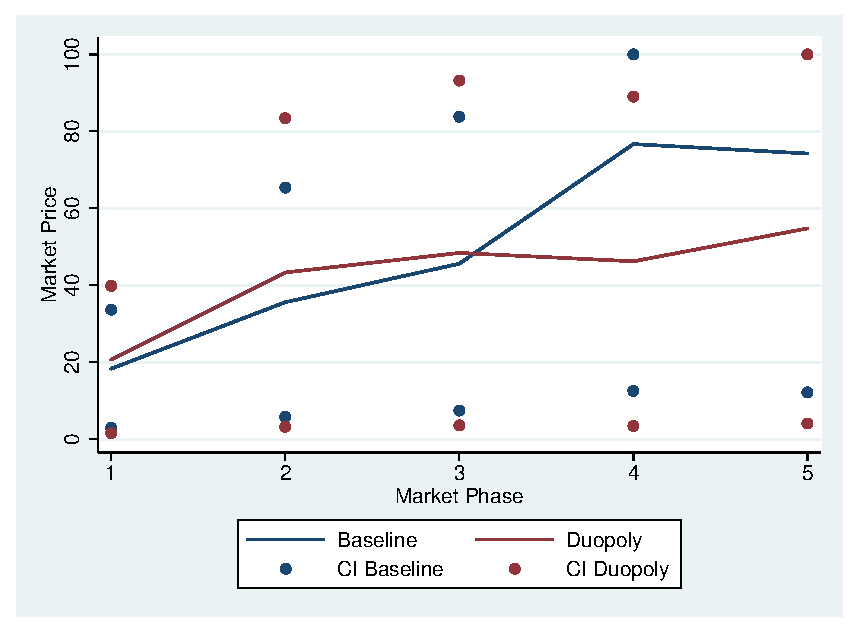
\includegraphics[width=0.9\linewidth]{market_price_over_period_mean.eps}
			\caption{Price by market phase}
		\end{subfigure}
	\end{figure}
	
\end{frame} 

%------------------------------------------------

\begin{frame}{Conclusion}
\framesubtitle{Discussion}			

	\begin{itemize}
		\item "Rich get richer"
		\item Dissassortative Network
		\item Starting point for future research
	\end{itemize}
\end{frame}

	


\end{document}


